\documentclass[14pt,a4paper]{article}
\usepackage{enumitem}
\usepackage{floatrow}
\usepackage{graphicx}
\usepackage[paperheight=25in,top=1in,bottom=1in,right=1in,left=1in,heightrounded]{geometry}
\usepackage{listings}
\usepackage{easylist}

\usepackage{graphicx,comment,framed}
\usepackage{amsthm,amssymb,amsmath}
%\usepackage[colorlinks,linkcolor=blue,citecolor=blue]{hyperref}

\usepackage{amssymb,amsmath}
\usepackage[colorlinks,linkcolor=blue,citecolor=blue]{hyperref}\usepackage{amsmath}
\usepackage{amsfonts}
\usepackage{amssymb}
\usepackage[usenames,dvipsnames]{pstricks}
\usepackage{graphicx,subfigure,wrapfig, relsize}
\usepackage{fancyhdr}
\usepackage[mathscr]{euscript}
\usepackage{multicol}

\usepackage{algorithmicx,algorithm}

\usepackage{xepersian}
\usepackage[noend]{algpseudocode}

%--------------------- page settings ----------------------

\settextfont[Scale=1.2]{XB Niloofar.ttf}
\setdigitfont[Scale=1.2]{XB Niloofar.ttf}
\defpersianfont\sayeh[Scale=1.2]{XB Kayhan Pook.ttf}
\addtolength{\textheight}{3.2cm}
\addtolength{\topmargin}{-22mm}
\addtolength{\textwidth}{2.7cm}
\addtolength{\oddsidemargin}{-1.5cm}



%-------------------------- Notations ------------------------------------

\newcommand{\IR}{\ensuremath{\mathbb{R}}} 
\newcommand{\IZ}{\ensuremath{\mathbb{Z}}} 
\newcommand{\IN}{\ensuremath{\mathbb{N}}} 
\newcommand{\IS}{\ensuremath{\mathbb{S}}} 
\newcommand{\IC}{\ensuremath{\mathbb{C}}} 
\newcommand{\IB}{\ensuremath{\mathbb{B}}} 

\newcommand{\bR}{\mathbb{R}}
\newcommand{\cB}{\mathcal{B}}
\newcommand{\cO}{\mathcal{O}}
\newcommand{\cG}{\mathcal{G}}
\newcommand{\rM}{\mathrm{M}}
\newcommand{\rC}{\mathrm{C}}
\newcommand{\rV}{\mathrm{V}}

\newcommand{\lee}{\leqslant}
\newcommand{\gee}{\geqslant}
\newcommand{\ceil}[1]{{\left\lceil{#1}\right\rceil}}
\newcommand{\floor}[1]{{\left\lfloor{#1}\right\rfloor}}
\newcommand{\prob}[1]{{\mbox{\tt Pr}[#1]}}
\newcommand{\set}[1]{{\{ #1 \}}}
\newcommand{\seq}[1]{{\left< #1 \right>}}
\newcommand{\provided}{\,|\,}
\newcommand{\poly}{\mbox{\rm poly}}
\newcommand{\polylog}{\mbox{\rm \scriptsize polylog}\,}
\newcommand{\comb}[2] {\left(\!\!\begin{array}{c}{#1}\\{#2}\end{array}\!\!\right)}

\newcommand{\REM}[1]{}
\newcommand{\mrbox}[1]{\mbox{\lr{#1}}}





%------------------------- Header -----------------------------

\newcommand{\سربرگ}[3]{
\def\ci{\perp\!\!\!\perp}
\hspace{16.5em}
\textbf{به نام خدا}
\parindent=0em
\vspace{0.5cm}

\rightline{
\makebox[6em][c]{

\includegraphics[height=1.6cm]{sharif.png}
}}
\vspace{-.2em}
{\scriptsize\bf دانشکده‌ی مهندسی کامپیوتر}
\hfill {\small
مدرس: دکتر احسان‌الدین عسگری 
}\\[-5em]
\leftline{\hfill\Large\bf 
پردازش زبان‌ طبیعی
}\\[.7em]
\leftline{\hfill\bf 
نیم‌سال دوم 02-01
}\\[1.7em]
\hrule height .12em

\normalsize
\vspace{1mm} #1
\hfill \small  #3
\vspace{1mm} 
\hrule height .1em

\vspace{-1.5em} 
\hfill {\sayeh\large #2} \hfill
}



\pagenumbering{gobble}
%\definecolor{ivory}{rgb}{1.0, 1.0, 0.94}
%\pagecolor{ivory} 
\usepackage{watermark}
\usepackage{transparent}
\usepackage{setspace}
\usepackage{xepersian}
\begin{document}
\vspace{0.5cm}	

\سربرگ{خلاصه جلسه هفته ۲-۱۳}{طبقه بندی متن}{ابوالفضل ملک احمدی}
\vspace{0.5cm}
\setstretch{2}	
\section{ classification}
\subsection{ ارزیابی}
\centerline{\text{برای ارزیابی از Cross-Validation استفاده میکنیم به این صورت که داده ها را به k بخش قسمت کرده}}
\\ 
\centerline{\text{ در هر که در هر بخش یک قسمت را به داده های test و مابقی را به داده های train  بخش بندی میکنیم }}
\\
\centerline{ \text{در نهایت مدلی که بیشترین میانگین و کمترین واریانس را دارد به عنوان بهترین مدل در نظر میگیریم}}
\\
*\text{معیار های ارزیابی عبارتند از :}

\centerline{$\text { Microf } 1=\sum_c \alpha_i f 1_c, \text { Macro } f 1=\frac{1}{|c|} \sum_c f 1_c$}

**\text{$\alpha_i$ بر اساس تعداد داده ها}
\\


*\text{سایر معیار های ارزیابی در شکل ۱ آمده اند.}


\centerline{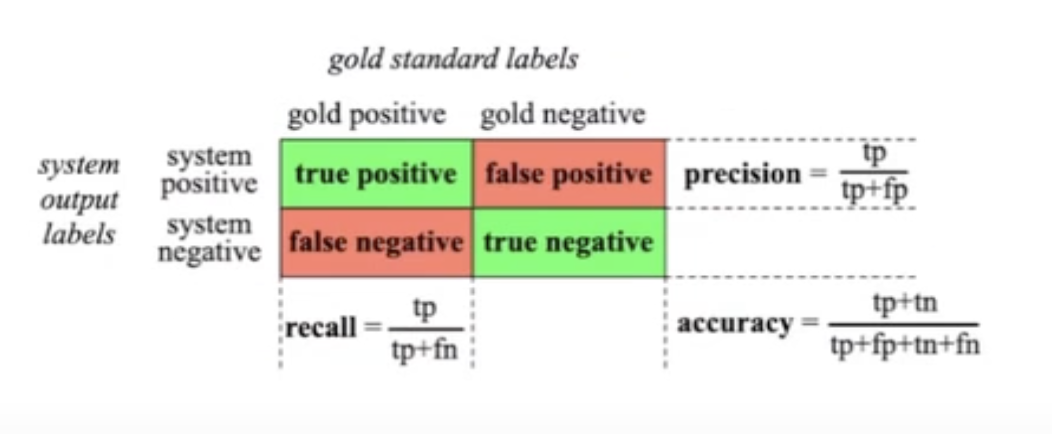
\includegraphics[scale=0.6]{LectureNoteTemplate/pics/met.png}}
\centerline{\caption{شکل۱:معیارهای ارزیابی}}
\subsection{ \text{\left Generative Classifiers - Naıve Bayes  }}

\centerline{$\text { Naive Buyes: } \hat{y}=\underset{y \in Y}{\operatorname{argmax}} P(y \mid x)=\underset{y \in Y}{\operatorname{argmax}} \frac{P(x \mid y) P(y)}{P(n) \leadsto \text { ignore }}$}
\\
\text{اگر حالت unigram در نظر بگیریم $\left.P(n \mid y)=\prod_{i=1}^n P (w_{v_i} \mid y\right) P(y)$}
\\
\text{و اگر  تعداد کلمات $|V|$ باشد برای یادگیری آن $2|V|+1$ پارامتر لازم داریم}


\subsection{\text{\left Discriminative Classifier - logistic regression}}

\begin{center}
    $ \rho(y=1)=\sigma(w \cdot x+b)=\hat{y}$  $w_{\cdot} x=\sum_{i=1} w_i x_i$ \\
    $ \rho(y=0)=1-\rho(y=1)=1-\hat{y}$
\end{center}
\begin{center}


    $ p\left(y(x)=\hat{y}^y \times(1-\hat{y})^{1-y}) \rightarrow-\log p(y \mid x)=-(y \log \hat{y}+(1-y) \log (1-\hat{y}))=L_{C E}\left(y, \hat{y}^{\prime}\right.\right). \rightarrow \text { crossentropy loss }  $\\
    برای جلو گیری از :overfitting\\
    $ \hat{\theta}=\underset{\theta}{\operatorname{argmax}} \sum_{i=1}^m \log p\left(y^i \mid x^i\right)-\underbrace{\alpha R(\theta)}_{\text {regularization }} R(\theta)=\left\{\begin{array}{l}$
   $ \|\theta\|_2^2=\sum \theta_i^2 \\$$
   $$ \|\theta\|_1=\sum\left|\theta_i\right|$
\end{array}\right. \\

\end{center}


\section{تحلیل sentiment}

**تحلیل احساسات جنبه های زیادی دارد و میتواند در سطح doc , token , ... بررسی شود 
$\\$
*\text{ بحث sentiment و  aspect   خیلی باهم آمیخته هستند ولی معمولا این دوتا رو باهم برچسب زده نداریم؛ }
$\\$
\text{به عبارت دیگر مثلا ما یک کلمه را نداریم که از یک منظر   برچسب  مثبت و از یک منظر برچسب منفی داشته باشه}
$\\$
*\text{راه های شناسایی تشخیص مثبت یا منفی بودن جمله عبارتند از :}
$\\$
\centerline{\text{۱.تعداد کلملات مثبت و منفی را می شماریم اگر تعداد مثبت ها بیشتر بود جمله مثبت و اگر تعداد منفی ها بیشتر بود جمله منفی .}}
\centerline{\text{مشکل: احتمال دارد تعداد مثبت و منفی یکی باشد در نتیجه جمله خنثی در نظر گرفته میشود}}
\centerline{\text{۲. استفاده از Naive Bayes که فقط  کلمات مثبت منفی را در نظر بگیریم یا کل کلمات رو در نظر بگیریم}}
\centerline{\text{۳.استفاده از Logistic Regression یا استفاده از neural network ها}}


\centerline{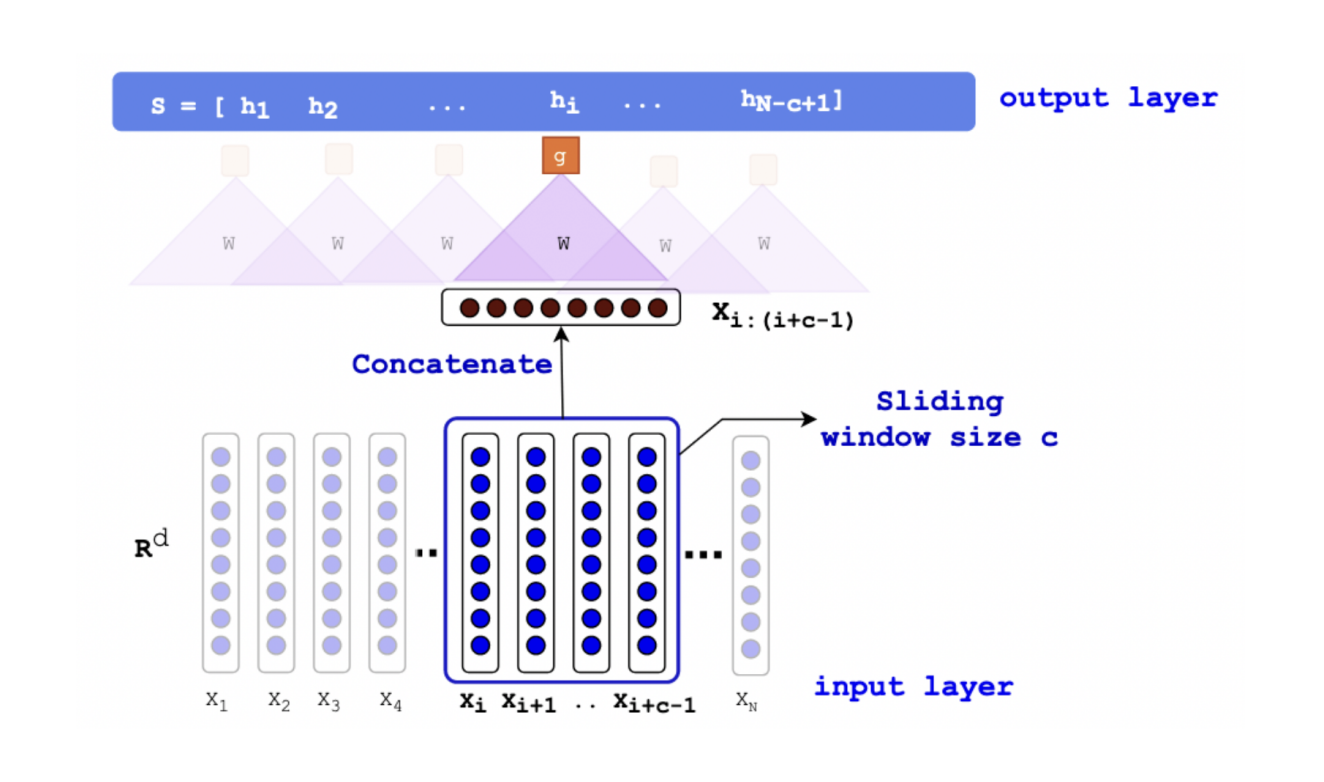
\includegraphics[scale=0.3]{LectureNoteTemplate/pics/cnn.png}}
\centerline{\caption{شکل۲:استفاده از cnn برای حل مسئله طبقه بندی}}


**\text{اگر Multiclass  بود از Softmax در تابع فعال سازی لایه اخر استفاده مکینم اگر multilabel 
 , Multiclass  بود از sigmoid .}
\watermark{\centering\put(350,-1720){
\includegraphics[scale=0.20]{pics/watermark3}}}
\end{document}